\documentclass[12pt]{beamer}
\usetheme{Frankfurt}
\usepackage[utf8]{inputenc}
\usepackage[english]{babel}
\usepackage{amsmath}
\usepackage{amsfonts}
\usepackage{amssymb}
\usepackage{booktabs}
% \author{Martin Dobiasch}
%\author{Martin \textsc{Dobiasch} \& Eugen \textsc{Havasi} \& Peter \textsc{Rjabcsenko}}
\author{Martin Dobiasch \& Eugen Havasi \& Peter Rjabcsenko}
%\title{}
%\setbeamercovered{transparent} 
%\setbeamertemplate{navigation symbols}{} 
%\logo{} 
%\institute{} 
%\date{} 
%\subject{} 
\begin{document}

\begin{frame}
\titlepage
\end{frame}

%\begin{frame}
%\tableofcontents
%\end{frame}

\begin{frame}{General Setup}
\begin{block}{Algorithms}

\end{block}

10 fold cross validation

Values reported are mean $\pm$ standard deviation

\end{frame}

\section{Communities}
\begin{frame}{Dataset}
Communities and Crime Data Set

Number of Instances: 1994

Number of Attributes: 128

Contains missing values

Task: Predict Violent Crimes per Population
\end{frame}

\begin{frame}{Initial view}
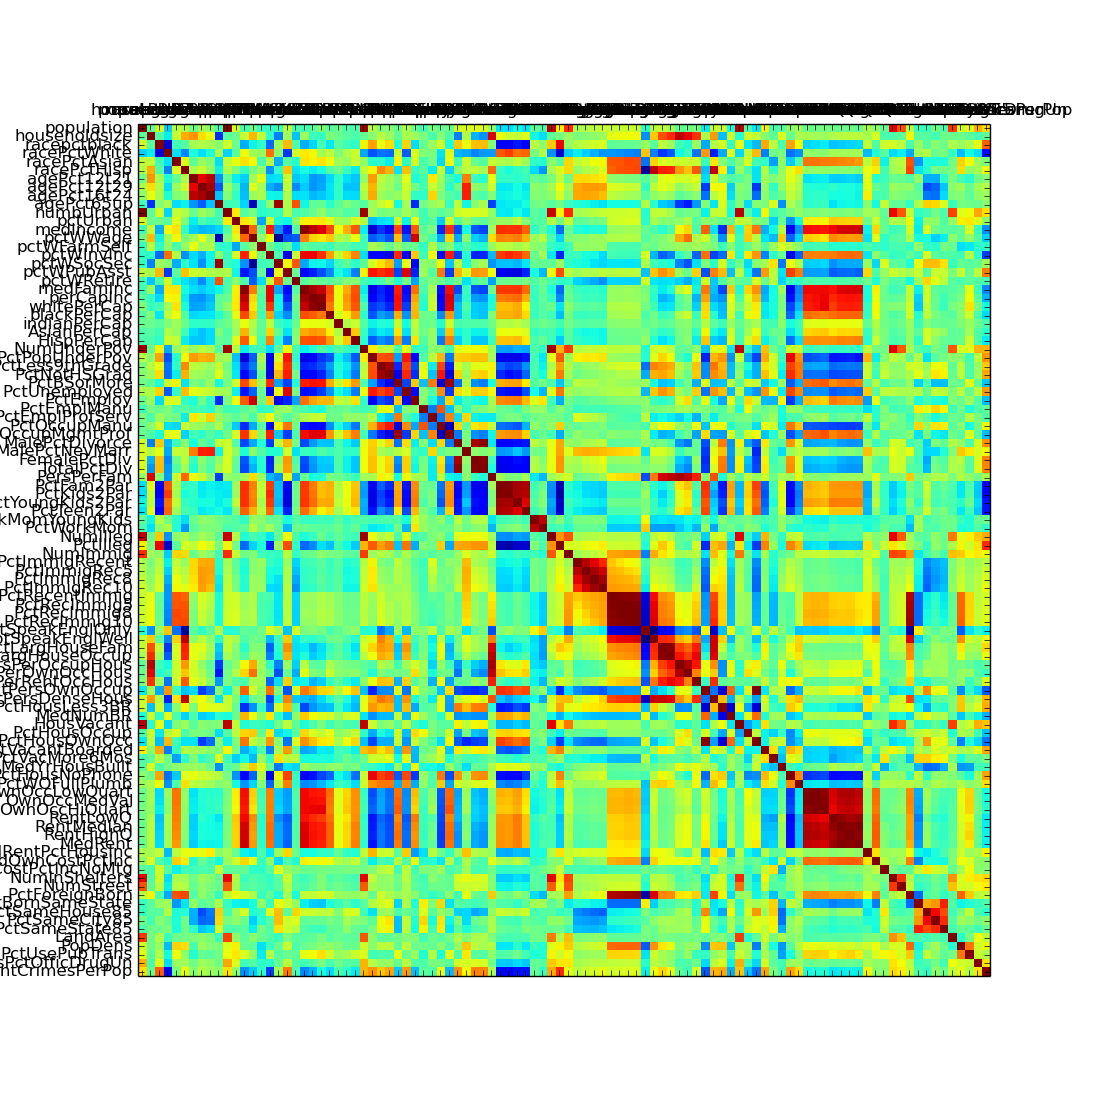
\includegraphics[height=\textheight,width=\textwidth,keepaspectratio]{plots/communities_orig.png}
\end{frame}

\begin{frame}{Preparations 1/2}
\begin{block}{Irrelevant}
state, county, community, communityname, fold

(from Dataset description)
\end{block}

\begin{block}{New Feature}
Recent Immigration: Split up 'recent', 'past 10', 'past 8', 'past 5' into '0 to 3', '3 to 5', '5 to 8', '8 to 10'
\end{block}
\end{frame}

\begin{frame}{Preparations 2/2}
\begin{block}{Side Notes}
''percentage of households with social security income in 1989''
correlates with ''percentage of population that is 65 and over in age''.

'percentage of people 16 and over who are employed in management or professional occupations'
correlates with ''percentage of people 25 and over with a bachelors degree or higher education''.
\end{block}

\begin{block}{After Cleaning}
Only 66 features left
\end{block}
\end{frame}

\begin{frame}{Final view}
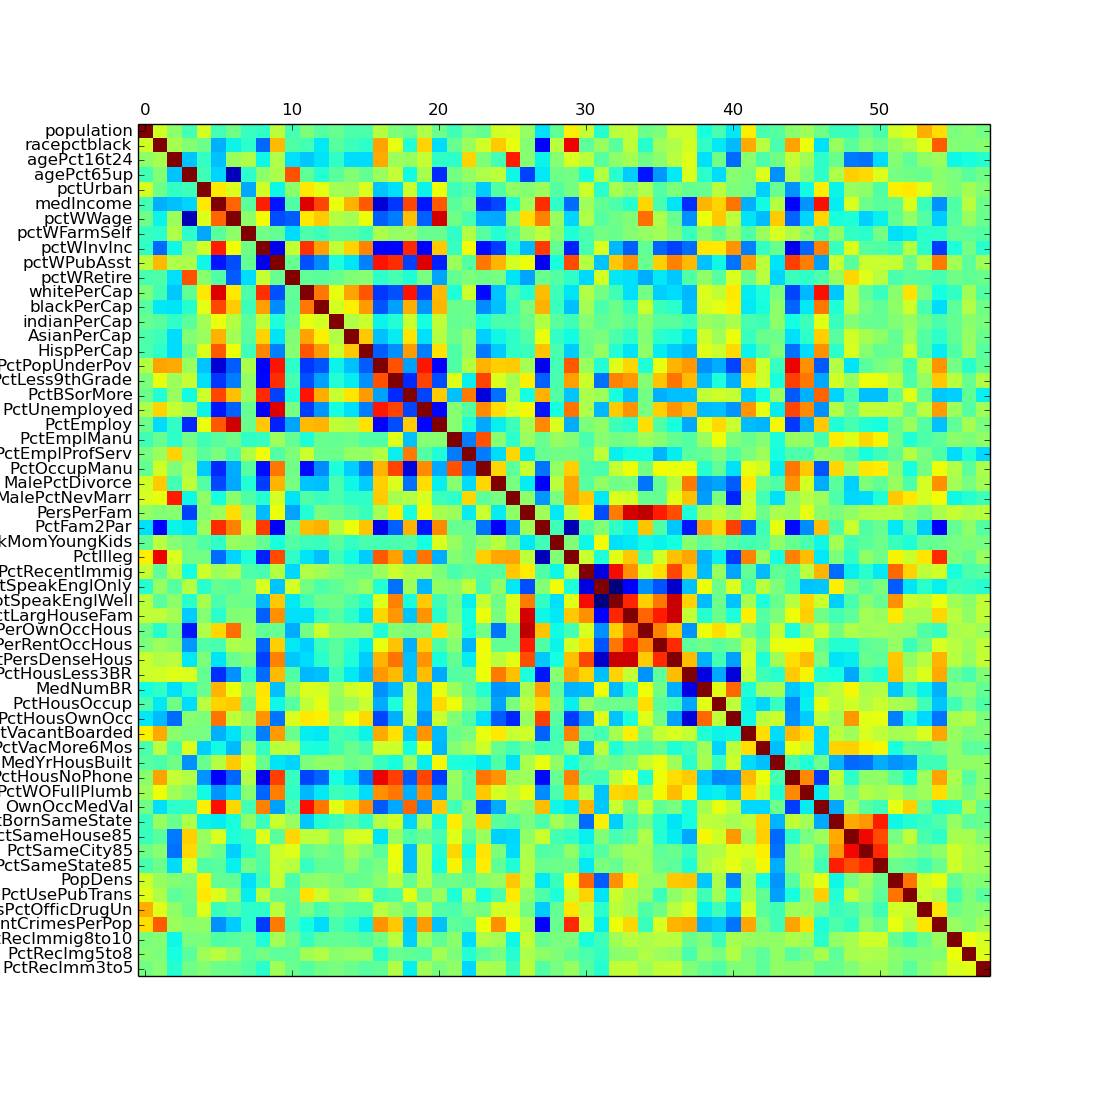
\includegraphics[height=\textheight,width=\textwidth,keepaspectratio]{plots/communities_final.png}
\end{frame}

\begin{frame}{Results}
\resizebox{\linewidth}{!}{\begin{tabular}{lrrrrr}
\toprule
\textbf{Algorithm/Setting} & \textbf{time (ms)} & \textbf{time p (ms)} & \textbf{rmse} & \textbf{mae} & \textbf{cv}\\
\midrule
GaussianNB & $571.39 \pm 437.55$ & $27.67 \pm 13.26$ & $0.62 \pm 2.96$ & $0.44 \pm 2.08$ & $0.00 \pm 0.00$\\
\bottomrule
\end{tabular}
}
\end{frame}

\section{Stock}
\begin{frame}{Dataset}
...

Number of Instances: 1994

Number of Attributes: 128

No missing values

Task: ?

4 periods of data $\rightarrow$ accumulated data
\end{frame}

\begin{frame}{Initial view}
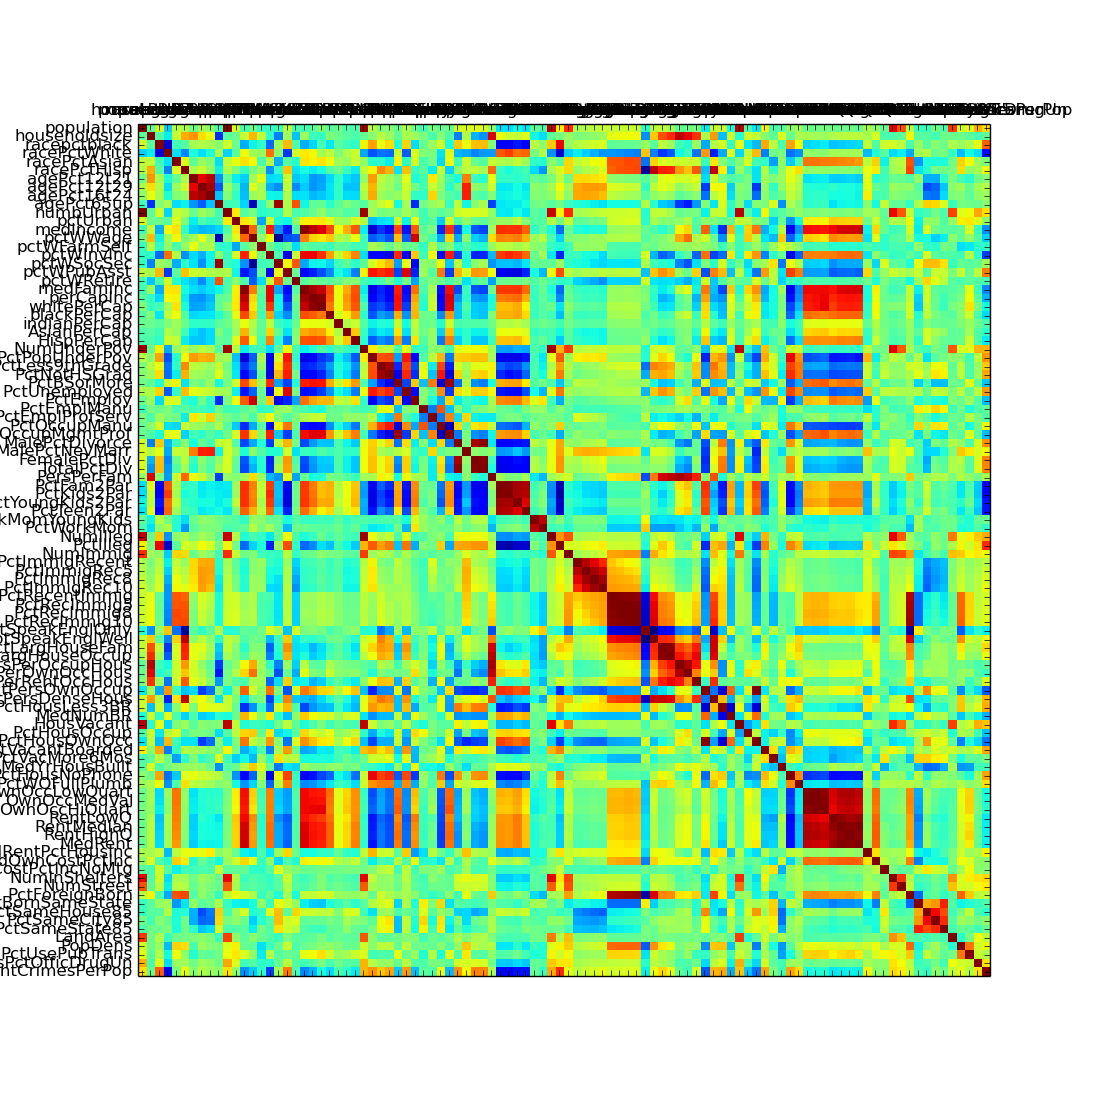
\includegraphics[height=\textheight,width=\textwidth,keepaspectratio]{plots/communities_orig.png}
\end{frame}

\section{Auto}
\begin{frame}{Initial view}
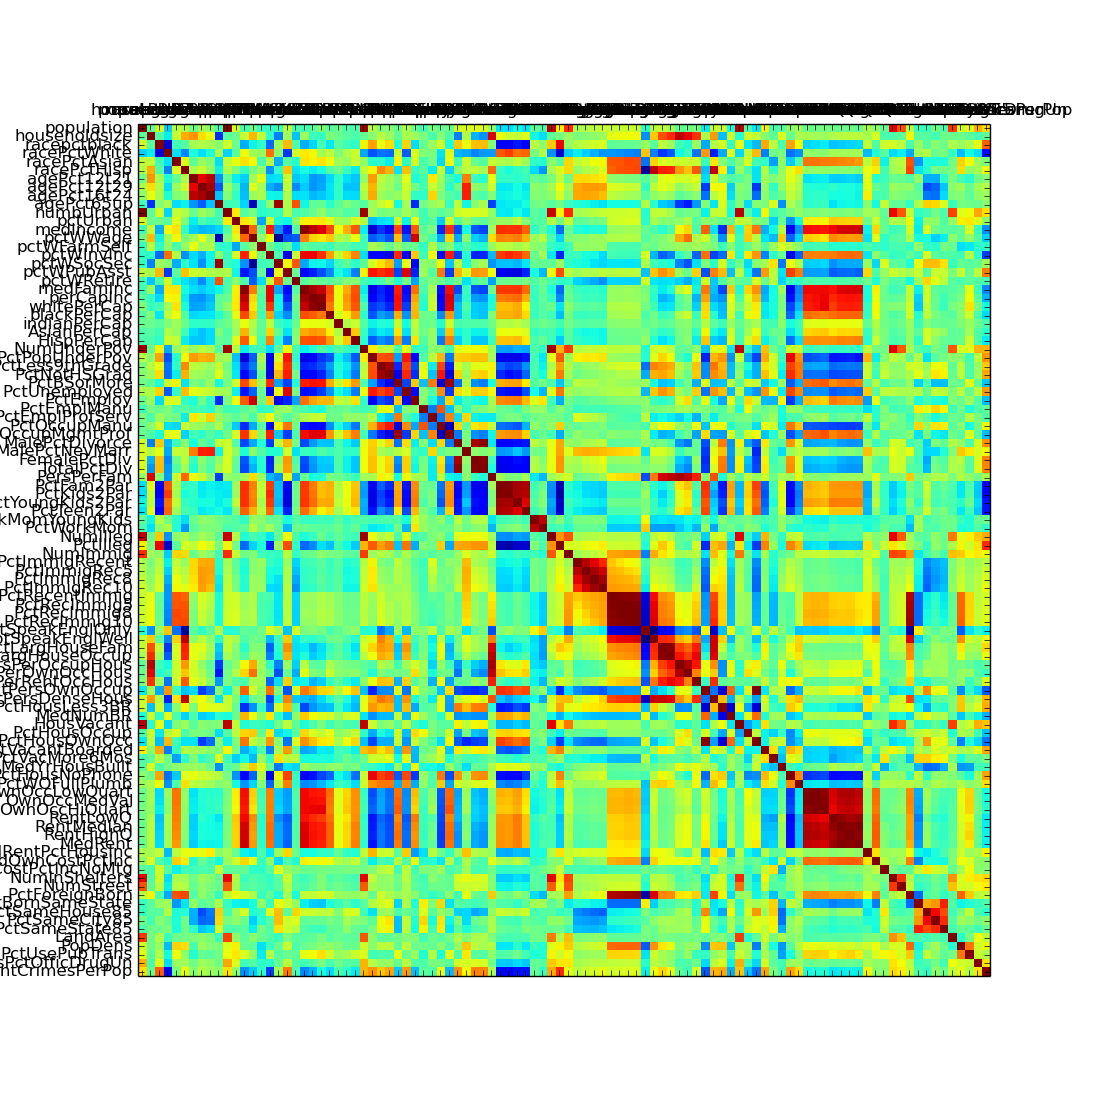
\includegraphics[height=\textheight,width=\textwidth,keepaspectratio]{plots/communities_orig.png}
\end{frame}

\section{KDD}
\begin{frame}{Initial view}
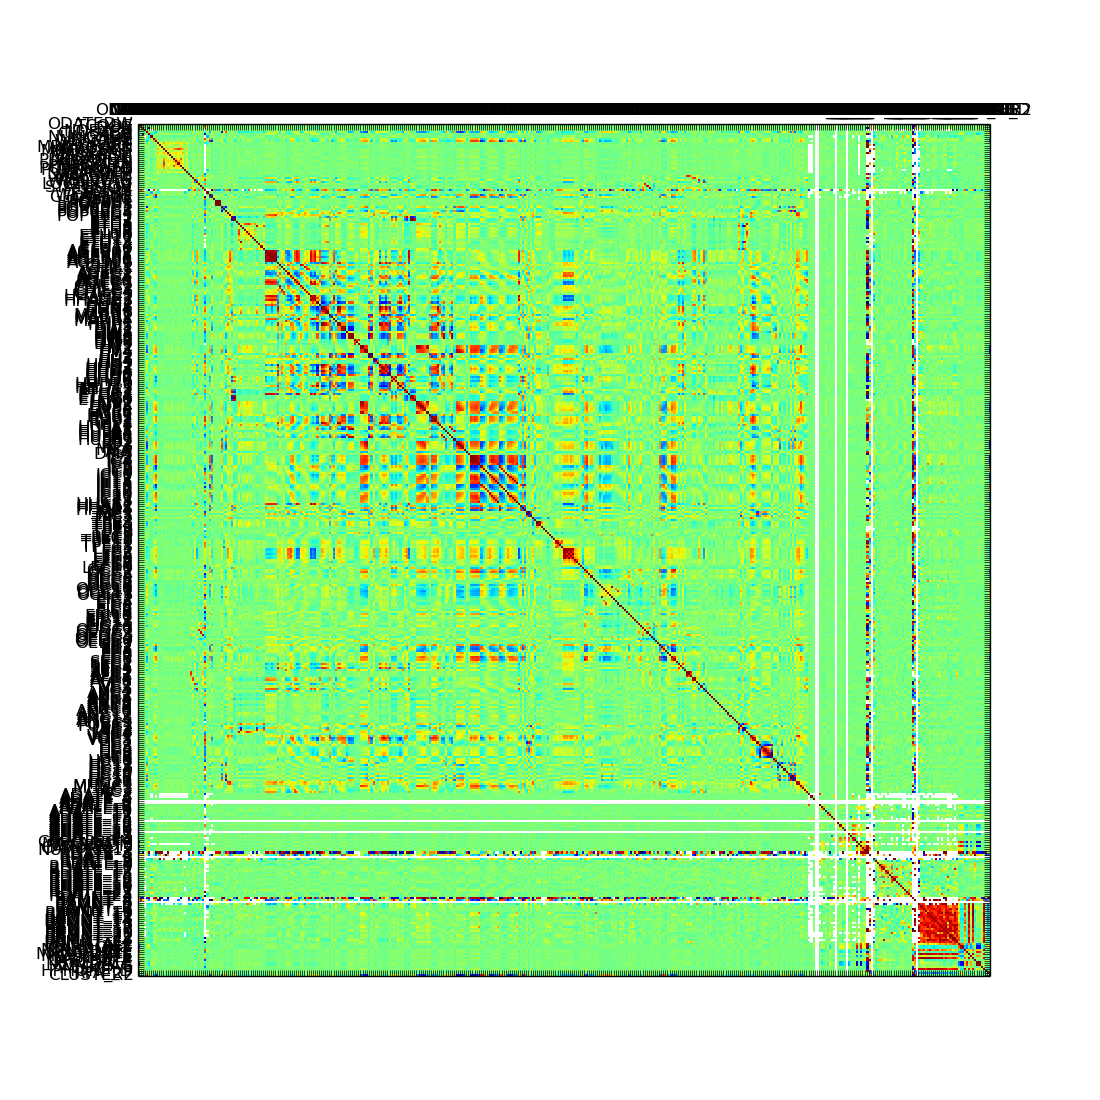
\includegraphics[height=\textheight,width=\textwidth,keepaspectratio]{plots/kdd_orig.png}
\end{frame}

\begin{frame}{Initial view}
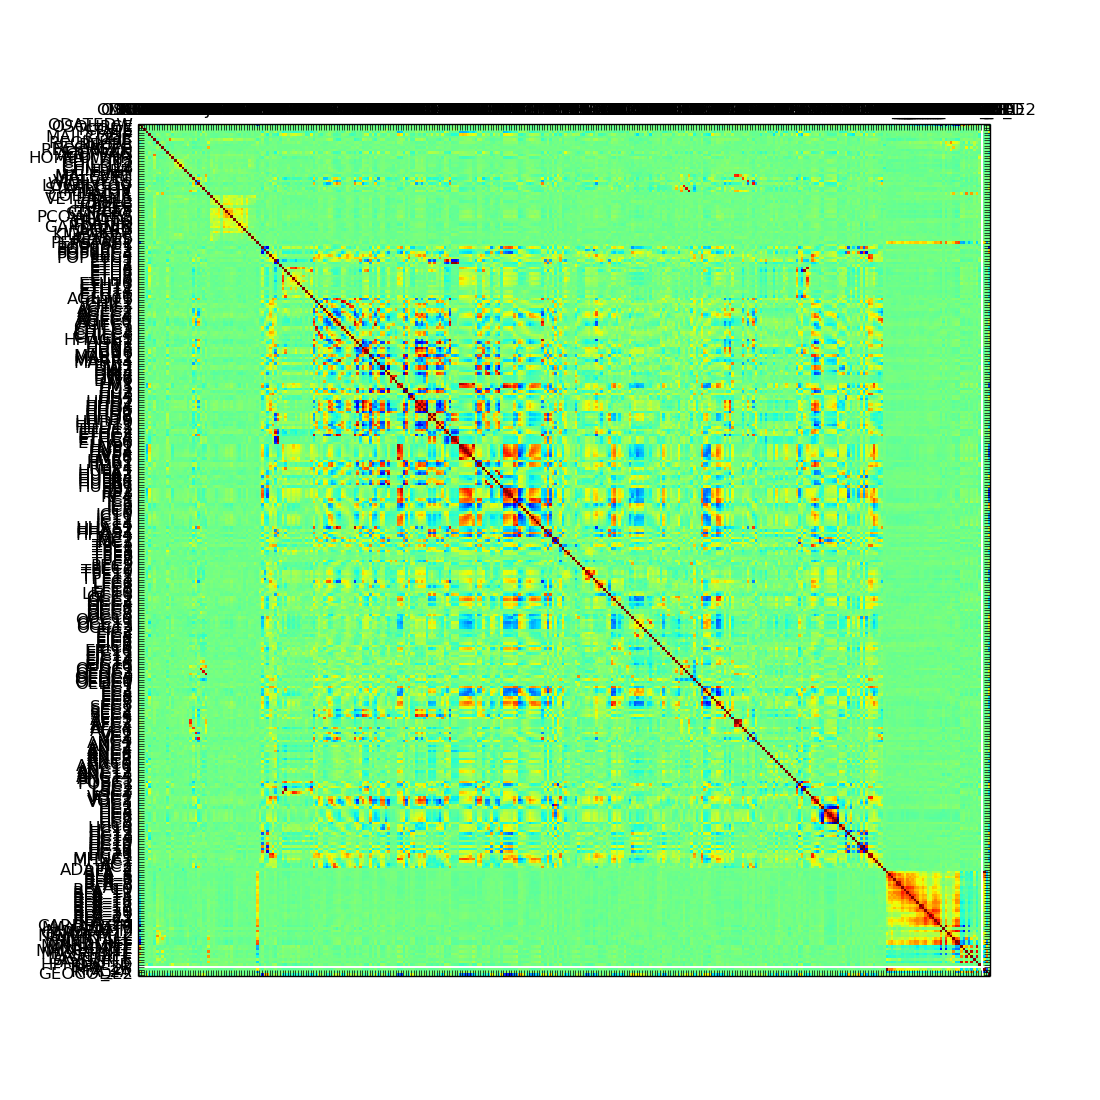
\includegraphics[height=\textheight,width=\textwidth,keepaspectratio]{plots/kdd_final.png}
\end{frame}

\begin{frame}{Findings}
Imputing mean vs. removing cols with missing values: latter gives better results
% results from removing:
% ({'n_neighbors': 291, 'p': 2, 'weights': 'uniform'}, 4.1350573536016384)
% ({'splitter': 'best', 'criterion': 'friedman_mse', 'max_features': 'auto'}, 4.1544598320715354)
% Results from imputing mean
% ({'n_neighbors': 291, 'p': 2, 'weights': 'uniform'}, 4.289451889295445)
% ({'splitter': 'best', 'criterion': 'friedman_mse', 'max_features': 'auto'}, 4.2979202497555358)
\end{frame}

\section{Summary}
\begin{frame}

No real runtime measurements
\end{frame}

\end{document}